\documentclass[sigconf]{acmart}

\usepackage{verbatim}

\usepackage{graphicx}				% Use pdf, png, jpg, or eps§ with pdflatex; use eps in DVI mode
								% TeX will automatically convert eps --> pdf in pdflatex		
\usepackage{amssymb}

\usepackage{algorithm}
\usepackage[noend]{algpseudocode}
\algrenewcommand\textproc{}
%\usepackage[boxed, linesnumbered]{algorithm2e}

\usepackage{array}

\usepackage{subfigure}

\usepackage{epstopdf}

\usepackage{multicol}

\usepackage{balance}

\usepackage{hhline}

%\newtheorem{theorem}{Theorem}%[section]
%\newtheorem{lemma}[theorem]{Lemma}
%\newtheorem{claim}[theorem]{Claim}
%\newtheorem{fact}[theorem]{Fact}
%\newtheorem{definition}[theorem]{Definition}
%\newtheorem{property}[theorem]{Property}

\newcommand{\sq}{\hbox{\rlap{$\sqcap$}$\sqcup$}}
%\newcommand{\qed}{\hspace*{\fill}\sq}

%\newenvironment{proof}{\noindent {\bf Proof.}\ }{\qed\par\vskip 4mm\par}
%\newenvironment{proofof}[1]{\bigskip \noindent {\bf Proof of #1:}\quad }{\qed\par\vskip 4mm\par}

\newcommand{\latpim} {\mathcal{L}_{pim}}
\newcommand{\latcpu} {\mathcal{L}_{cpu}}
\newcommand{\latllc} {\mathcal{L}_{llc}}
\newcommand{\latato} {\mathcal{L}_{atomic}}
\newcommand{\latmes} {\mathcal{L}_{message}}
\newcommand{\Sp}{\mathcal{S}_{p}}


\usepackage{booktabs} % For formal tables


\copyrightyear{2017}
\acmYear{2017}
\setcopyright{acmcopyright}
\acmConference{SPAA '17}{July 24-26, 2017}{Washington DC, USA}
\acmPrice{15.00}
\acmDOI{http://dx.doi.org/10.1145/3087556.3087582}
\acmISBN{978-1-4503-4593-4/17/07}

\clubpenalty = 10000
\widowpenalty = 10000

\begin{document}\sloppy

\title{Concurrent Data Structures for Near-Memory Computing}


\author{Zhiyu Liu}
\affiliation{%
  \institution{Computer Science Department\\
Brown University}
}
\email{zhiyu\_liu@brown.edu}

\author{Irina Calciu}
\affiliation{%
  \institution{VMware Research Group}
}
\email{icalciu@vmware.com}

\author{Maurice Herlihy}
\affiliation{%
  \institution{Computer Science Department\\
Brown University}
}
\email{mph@cs.brown.edu}

\author{Onur Mutlu}
\affiliation{%
  \institution{Computer Science Department\\
ETH Zurich}
}
\email{onur.mutlu@inf.ethz.ch}

% The default list of authors is too long for headers}
%\renewcommand{\shortauthors}{B. Trovato et al.}


\begin{abstract}

The performance gap between memory and CPU has grown exponentially. 
To bridge this gap, hardware architects have proposed 
near-memory computing (also called processing-in-memory, or PIM), 
where a lightweight processor (called a PIM core) is located close to 
memory. 
Due to its proximity, a memory access from a PIM core is much faster than from a CPU core.
New advances in 3D 
integration and in die stacked memory make PIM viable in the 
near future. Prior work has shown significant performance improvements by using PIM for 
embarrassingly parallel and data-intensive applications, as well as for
pointer-chasing traversals in \emph{sequential} data structures. 
However, current server machines have hundreds of cores; algorithms for 
concurrent data structures exploit these cores to achieve high throughput and 
scalability, with significant benefits over sequential data structures. 

In this paper, we show that
  naive PIM data structures cannot outperform 
 state-of-the-art \emph{concurrent} data structures. 
We 
investigate two classes of data structures. First, we analyze pointer chasing data 
structures, which have a high degree of inherent parallelism and low contention, but incur significant 
overhead due to unpredictable memory accesses. Second, we explore
FIFO queues, which can leverage CPU caches to exploit their inherent high locality, but have a high degree of contention. 
We propose new designs for PIM 
data structures using 
techniques such as combining, partitioning and pipelining, that can outperform traditional 
concurrent data structures, with a significantly simpler design. 


\end{abstract}


%
% The code below should be generated by the tool at
% http://dl.acm.org/ccs.cfm
% Please copy and paste the code instead of the example below.
%
%\begin{CCSXML}
%\end{CCSXML}

\keywords{concurrent data structures; parallel programs; processing-in-memory; near-memory computing}

\maketitle

%\section{Introduction}
\section{Near-memory Computing}

The performance gap between memory and CPU has grown exponentially. 
Memory vendors have focused mainly on improving memory capacity and bandwidth, 
sometimes even at the cost of increased memory access latencies 
\cite{Chang:2016, DBLP:conf/hpca/LeeKPKSCM15}. 
To provide higher bandwidth with lower access latencies, hardware architects 
have proposed near-memory computing (also called \textit{processing-in-memory}, 
or PIM), where a lightweight processor (called a PIM core) is located close to 
memory. A memory access from a PIM core is much faster than that from a CPU 
core. 
Near-memory computing is an old idea that has been intensely studied in the 
past (e.g., 
\cite{Stone1970, Kogge1994, Gokhale1995, Patterson1997, Oskin1998, 
KangHYKGLTP99, Hall1999, Elliott:1992}), 
but so far has not yet materialized. However, new advances in 3D integration and 
in die-stacked memory 
likely make near-memory computing viable in the near future. 
For example, one PIM design \cite{Ahn2015:2, Zhang2014:TTP, Ahn2015:1, boroumand2016} assumes 
that 
memory is organized in multiple vaults, each having an in-order PIM core to 
manage it. 
These PIM cores can communicate through message passing, but do not share memory, 
and cannot access each other's vaults. 

This new technology promises to revolutionize the interaction between 
computation and data, 
as it enables memory to become an active component in managing the data. 
Therefore, it invites a fundamental rethinking of basic data structures and 
promotes a tighter dependency between algorithmic design and hardware 
characteristics. 

Prior work has already shown significant performance improvements by using PIM 
for embarrassingly parallel 
and data-intensive applications~\cite{Zhang2014:TTP, Ahn2015:2, ZhuASSHPF13, 
Akin2015:DRM, Hsieh:2016:TOM}, 
as well as for pointer-chasing traversals~\cite{hsieh2016accelerating} in 
\emph{sequential} data structures. 
However, current server machines have hundreds of cores; 
algorithms for concurrent data structures exploit these cores to achieve high 
throughput and scalability, 
with significant benefits over sequential data structures 
(e.g., \cite{practicallf, skiplists-concpugh, valois, Herlihy08}).
Unlike prior work, we focus on \emph{concurrent} data structures for PIM 
and we show that naive PIM data structures \emph{cannot} outperform 
state-of-the-art concurrent data structures. 
In particular, the lower-latency access to memory provided by PIM cannot 
compensate 
for the loss of parallelism. 
For example, even if a PIM memory access is two times faster than a CPU memory access, a 
sequential PIM linked-list is still slower than a traditional concurrent linked-list accessed in parallel by only three 
CPU cores.

Therefore, to be competitive with traditional concurrent data structures, 
PIM data structures need new algorithms and new approaches to leverage 
parallelism.  
As the PIM technology approaches fruition, it is crucial to investigate how to 
best utilize it to exploit the lower latencies, while still using the vast amount of previous research 
related to concurrent data structures. 

In this paper, we provide answers to the following questions. 
How do we design and optimize data structures for PIM? And, how do these 
optimized PIM data structures compare to traditional CPU-managed concurrent data structures? To 
answer these questions, even before the hardware becomes available, we develop a 
simplified model of the expected performance of PIM. Using this model, we 
investigate two classes of data structures. 

First, we analyze \emph{pointer chasing data structures} (Section 
\ref{section:pointer_chasing}), 
which have a high degree of inherent parallelism and low contention, 
but which incur significant overhead due to hard-to-predict memory access patterns. 
We propose using techniques such as combining and partitioning 
the data across vaults to reintroduce parallelism for these data structures.

Second, we explore \emph{contended data structures} (Section 
\ref{section:contended}), such as FIFO queues, 
which can leverage CPU caches to exploit their inherent high locality. 
Therefore, FIFO queues might not seem to be able to leverage PIM's faster memory 
accesses. 
Nevertheless, these data structures exhibit a high degree of contention, which 
makes it difficult even for 
the most advanced data structures to obtain good performance when many threads access 
the data concurrently. 
We use pipelining of requests, which can be done very efficiently in PIM, to 
design a new FIFO queue 
suitable for PIM that can outperform state-of-the-art concurrent FIFO 
queues~\cite{Morrison13, Hendler10}.

The contributions of this paper are as follows:
\begin{itemize}
\item We propose a simple and intuitive model to analyze the performance of PIM data 
structures and of 
concurrent data structures. This model considers the number of atomic operations, the number of 
memory accesses and the number of accesses that can be served from the CPU cache. 
\item Using this model, we show that the lower-latency memory accesses provided 
by PIM 
are not sufficient for sequential PIM data structures to outperform efficient traditional concurrent 
data structures.
 \item We propose new designs for PIM data structures using 
techniques such as combining, partitioning and pipelining.
Our evaluations show that these new PIM data structures can outperform 
traditional 
concurrent data structures, with a significantly simpler design. 
\end{itemize}

The paper is organized as follows. In Section~\ref{section:hardware_model}, we 
briefly describe 
our assumptions about the hardware architecture. 
In Section~\ref{section:performance_model}, we introduce a simplified performance 
model 
that we use throughout this paper to estimate the performance of our data structures using 
the hardware 
architecture described in Section~\ref{section:hardware_model}. 
In Sections~\ref{section:pointer_chasing} and \ref{section:contended}, 
we describe and analyze our PIM data structures and use our model to compare 
them to prior work. 
We also use current DRAM architectures to simulate the behavior of our 
data structures and 
evaluate them compared to state-of-the-art concurrent data structures. 
Finally, we present related work in Section~\ref{section:related_work} 
and conclude in Section~\ref{section:conclusion}. 


%\section{Processing in Memory}
%\label{section:model}
\section{Hardware Architecture}


%\subsection{Hardware model}
\label{section:hardware_model}

\begin{figure}[ht!]
%$\hrulefill$
%\\
%\\
\centering
\includegraphics[width=.9\linewidth]{model.eps}
%$\hrulefill$
\caption{The PIM Architecture}
\label{figure:model}
\end{figure}

In an architecture utilizing PIM memory, multiple CPUs are connected to the main
memory, via a shared crossbar network, as illustrated in Figure \ref{figure:model}.
The main memory consists of two parts---one is a normal DRAM accessible by CPUs 
and the other, called the \textit{PIM memory}, is divided into multiple partitions, 
called \textit{PIM vaults} or simply vaults.  
According to the \textit{Hybrid Memory Cube} specification 1.0 \cite{website:HMC}, 
each HMC consists of 16 or 
32 vaults and has total size 2GB or 4 GB (so each vault has size roughly 100MB) 
\footnote{These small sizes are preliminary, and it is expected that each vault will be bigger when the 
PIM memory will be commercialized}. 
We assume the same specifications in our PIM model, although the size of a PIM memory and 
the number of its vaults can be bigger. 
Each CPU core also has access to a hierarchy of L1 and L2 caches backed by DRAM,
and a last level cache shared among multiple cores. 

Each vault has a \textit{PIM core} directly attached to it.
We say a vault is \textit{local} to the PIM core attached to it, and vice versa.
A PIM core is a lightweight CPU that may be slower than a full-fledged CPU
with respect to computation speed. 
A PIM core can be thought of as an in-order CPU with a small private L1 cache.
A vault can be accessed only by its local PIM core.\footnote{
We may alternatively assume that a PIM core has direct access to remote vaults, at a larger cost. 
We may also assume that vaults are accessible by CPUs as well, 
but at the cost of dealing with cache coherence between CPUs and PIM cores. 
Some cache coherence mechanisms for PIM memory claim to be not costly 
(e.g., \cite{boroumand2016, Ahn2015:1}). 
However, we prefer to keep the hardware model simple and we will show that we are still able to 
design efficient concurrent data structures with this simple, less powerful PIM memory.}
Although a PIM core is relatively slow computationally, it has fast access to its local vault.

A PIM core communicates with other PIM cores and CPUs via messages.
Each PIM core, as well as each CPU, has buffers for storing incoming messages.
A message is guaranteed to eventually arrive at the buffer of its receiver.
Messages from the same sender to the same receiver are delivered in FIFO order: 
the message sent first arrives at the receiver first. 
However, messages from different senders or to different receivers can arrive in an arbitrary order. 

We assume that a PIM core can only make read and write operations 
to its local vault, while a CPU also supports more powerful atomic operations, such as \emph{Compare-And-Swap (CAS)} 
and \emph{Fetch-And-Increment (F$\&$A)}.
Virtual memory can be realized efficiently if  
each PIM core maintains its own page table for the local vault~\cite{hsieh2016accelerating}.
\subsection{Performance model}
\label{section:performance_model}
Based on the latency numbers in prior work on PIM memory, 
in particular on the Hybrid Memory Cube \cite{website:HMC, Azarkhish16}, 
and on the evalutation of operations in multiprocessor architectures \cite{David13},
we propose the following simple performance model to compare 
our PIM-managed algorithms with existing concurrent data structure algorithms.
For read and write operations, we assume 
$$\latcpu = 3\latpim = 3\latllc,$$
where $\latcpu$ is the latency of a memory access by a CPU,
$\latpim$ is the latency of a local memory access by a PIM core, and
$\latllc$ is the latency of a last-level cache access by a CPU.
We ignore the costs of cache accesses of other levels in our performance model,
as they are negligible in the concurrent data structure algorithms we will consider.
We assume that the latency of a CPU making an atomic operation, such as a CAS or a F\&A,
to a cache line is 
$$\latato = \latcpu,$$ 
even if the cache line is currently in cache.
This is because an atomic operation hitting the cache is usually 
as costly as a memory access by a CPU, acorrding to \cite{David13}.
When there are $k$ atomic operations competing for a cache line concurrently,
we assume that they are executed sequentially, that is,
they complete in times $\latato, 2\latato,..., k\latato$, respectively.

We assume that the size of a message sent by a PIM core or a CPU is at most 
the size of a cache line.
Given that a message transferred between a CPU and a PIM core goes through
the crossbar network, we assume that the latency for a message to arrive at its receiver is 
$$\latmes = \latcpu.$$
We make a conservative assumption that the latency of a message transferred 
between two PIM cores is also $\latmes$.
Note that the message latency we consider here is the transfer time of a message
through a message passing channel, that is, the period between the moment
when a PIM or a CPU sends off the message and the moment when
the message arrives at the buffer of its receiver.
We ignore the time spent in other parts of a message passing procedure,
such as preprocessing and constructing the message,
as it is negligible compared to the time spent in message transfer.



%\section{Pointer-Chasing Data Structures}
\section{Data Structures with Low Contention}
\label{section:pointer_chasing}
Now we discuss how we design efficient PIM-managed pointer-chasing data structures.
In a pointer-chasing data structure, an operation (e.g., an insertion) has to traverse over 
items of the data structure by following a sequence of pointers, 
until it finds the right place to apply itself.
The examples we consider are linked-list and skip-list,
where add($x$), delete($x$) and contains($x$) operations have to go through
a sequence of ``next node" pointers until reaching the position of node $x$.
The performance bottleneck of such an operation is usually the pointer chasing procedure.
Here we focus on data structures much larger than the size of cache of CPUs
such that a large portion of a data structure has to reside in memory at any time.
Thus, the performance bottleneck becomes the memory accesses incurred during pointer chasing.


%\subsection{PIM-managed linked-list}
\subsection{Linked-lists}
\label{section:linked_list}
The naive PIM-managed linked-list is simple:
the linked-list is stored in a vault, maintained by the local PIM core.
Whenever a CPU\footnote{From now on, we use threads and CPUs interchangeably.} 
wants to make an operation to the linked-list,
it sends the PIM core a message containing a request of the operation. 
The PIM core will retrieve the message, execute the operation, and send the result back to CPU.
The concurrent linked-list can actually be implemented
as a sequential one, since it is accessible directly only by the PIM core.

Doing pointer chasing on sequential data structures by PIM cores is not a new idea
(e.g., \cite{hsieh2016accelerating, Ahn2015:2}).
It is obvious that for a sequential data structure like a sequential linked-list,
replacing the CPU with a PIM core to access the data structure will largely improve
its performance due to the PIM core's much faster memory access.
However, we are not aware of any prior comparison between the performance of
PIM-managed data structures and concurrent data structures
in which CPUs can make operations in parallel.
In fact, our analytical and experimental results will show that
the performance of the naive PIM-managed linked-list is much worse than
that of the concurrent linked-list with fine-grained locks \cite{Heller05}.

To improve the performance of the PIM-managed linked-list,
we apply the following \textit{combining optimization} to it:
the PIM core retrieves all pending requests from its buffer and
executes all of them during only one traversal over the linked-list.
It is not hard to see that the role of the PIM core in our PIM-managed linked-list
is very similar to that of the combiner in a concurrent linked-list implemented
using \textit{flat combining} \cite{Hendler10}, where, roughly speaking,
threads compete for a ``combiner lock" to become the combiner, and
the combiner will take over all operation requests from other threads and execute them.
Therefore, we think the performance of the flat-combining linked-list is a good indicator to
the performance of our PIM-managed linked-list.

Based on our performance model, we can calculate the approximate expected
throughputs of the linked-list algorithms mentioned above, 
when there are $p$ CPUs making operation requests concurrently.
We assume that a linked-list consists of nodes with integer keys in the range of $[1, N]$.
Initially a linked-list has $n$ nodes with keys generated independently
and uniformly at random from $[1, N]$.
The keys of the operation requests are generated the same way.
To simplify the analysis, we assume that CPUs only make $contains()$ requests
(or the number of $add()$ requests is the same as the number of $delete()$
so that the size of each linked-list nearly doesn't change).
We also assume that a CPU makes a new operation request immediately after
its previous one completes.
The approximate expected throughputs (per second) of the concurrent linked-lists
are listed below, given $n \gg p$ and $N \gg p$: 
\begin{itemize}
\item Concurrent linked-list with fine-grained locks:
	${2p \over (n+1)\latcpu}$

\item Flat-combining linked-list without combining optimization:
	${2 \over (n+1)\latcpu}$

\item PIM-managed linked-list without combining optimization:
	${2 \over (n+1)\latpim}$

\item Flat-combining linked-list with combining optimization:
    ${p \over (n-\Sp)\latcpu}$

\item PIM-managed linked-list with combining optimization:
    ${p \over (n-\Sp)\latpim}$
\end{itemize}
where $\Sp = \sum\limits_{i=1}^{n} ({i \over n+1})^{p}$.\footnote{
We define the rank of an operation request to a linked-list as the number of pointers
it has to traverse until it finds the right position for it in the linked-list.
$\Sp$ is the expected rank of the operation request with the biggest key
among $p$ random requests a PIM core or a combiner has to combine,
which is essentially the expected number of pointers a PIM core or a combiner
has to go through during one pointer chasing procedure.} 
It is easy to see that the PIM-managed linked-list with combining outperforms 
the linked-list with fine-grained locks, which is the best one among other algorithms, 
as long as ${\latcpu \over \latpim} > {2(n - \Sp)\over n + 1}$.
Given that $0 < \Sp \le {n \over 2}$ and $\latcpu = 3\latpim$,
the throughput of the PIM-managed linked-list with combining should be at least 
1.5 times the throughput of the linked-list with fine-grained locks.
Without combining, however, the PIM-managed linked-list cannot
beat the linked-list with fine-grained locks when $p > 6$.

We implemented the linked-list with fine-grained locks
and the flat-combining link-list with and without the combining optimization.
We ran them on a machine of 28 hardware threads
and their throughputs are presented in Figure \ref{figure:linkedlist_data}.
The results confirmed the validity of our analysis above.
The throughput of the flat-combining algorithm without combining optimization
is much worse than the algorithm with fine-grained locks.
Since we believe the performance of the flat-combining linked-list is a good 
indicator of that of the PIM-managed linked-list, we triple the throughput of the
flat-combining algorithm without combining optimization to get the estimated
throughput of the PIM-managed algorithm. 
As we can see, it is still far below the throughput of the one with fined-grained locks.
However, with the combining optimization, the performance of the flat-combining
algorithm improves significantly and the estimated throughput of our PIM-managed
linked-list with combining optimization now beats all others'.



\begin{figure}
    \centering
    \begin{minipage}{0.45\textwidth}
        \centering
        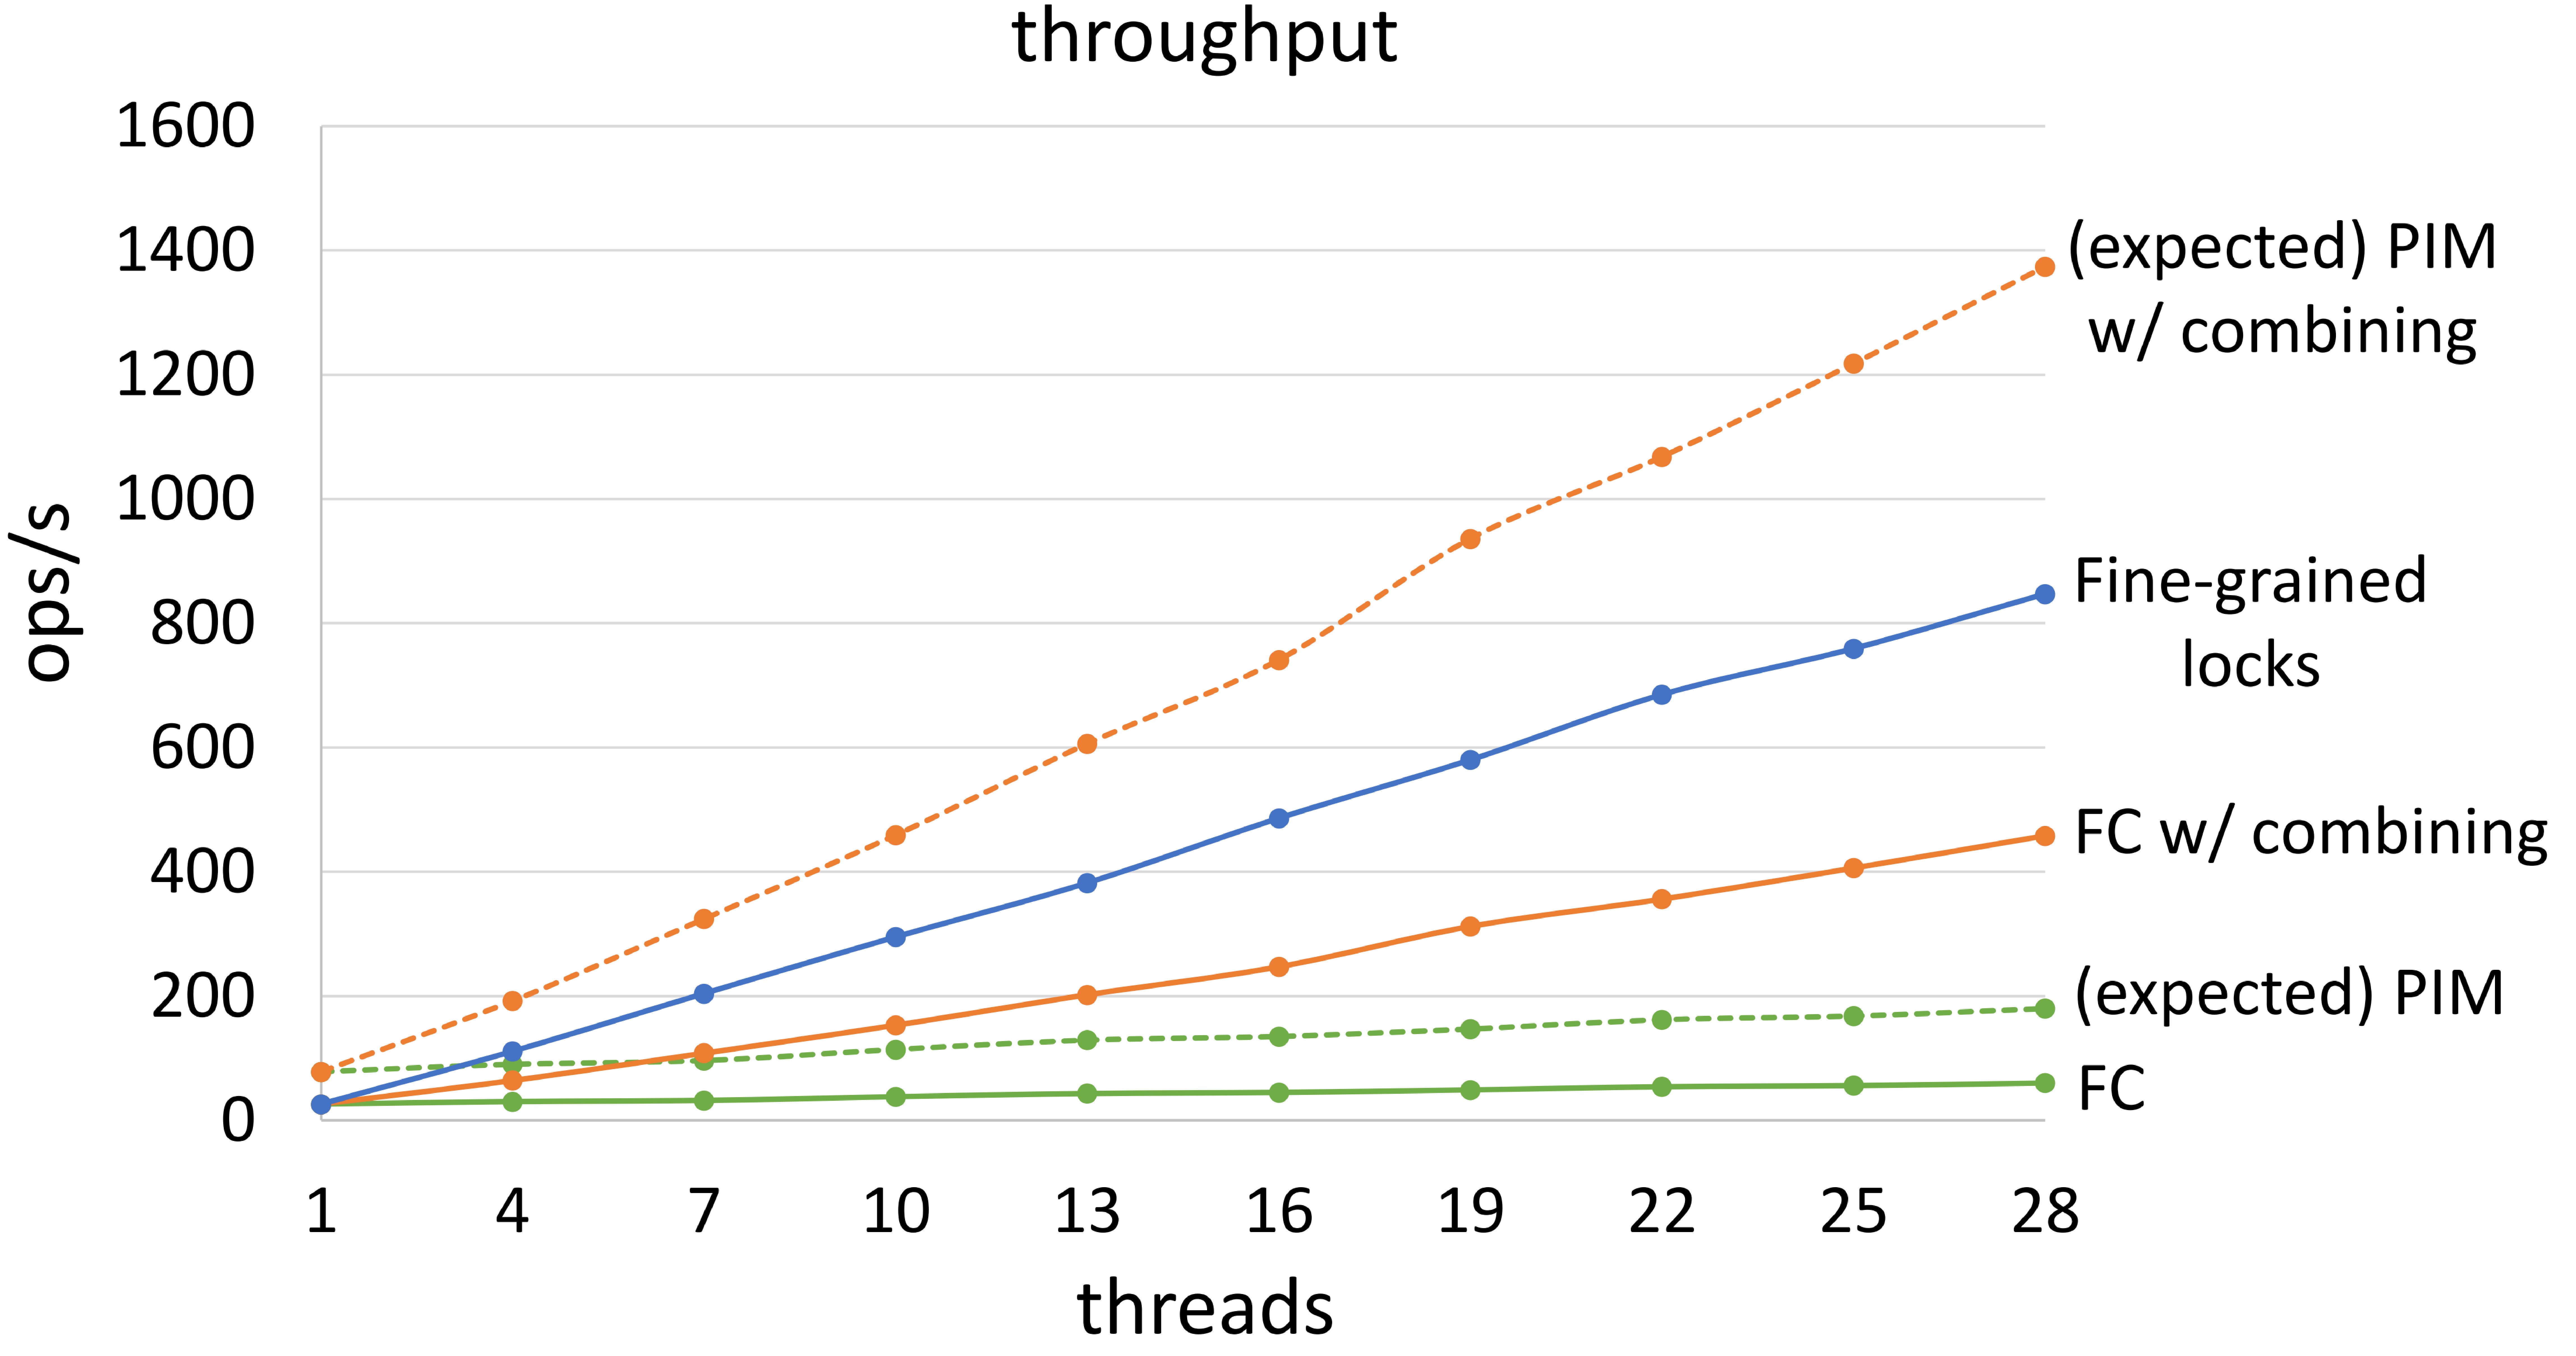
\includegraphics[width=.9\textwidth]{linkedlist_data.eps} % first figure itself
        \caption{Experimental results of linked-lists}
        \label{figure:linkedlist_data}
    \end{minipage}\hfill
    \begin{minipage}{0.45\textwidth}
        \centering
        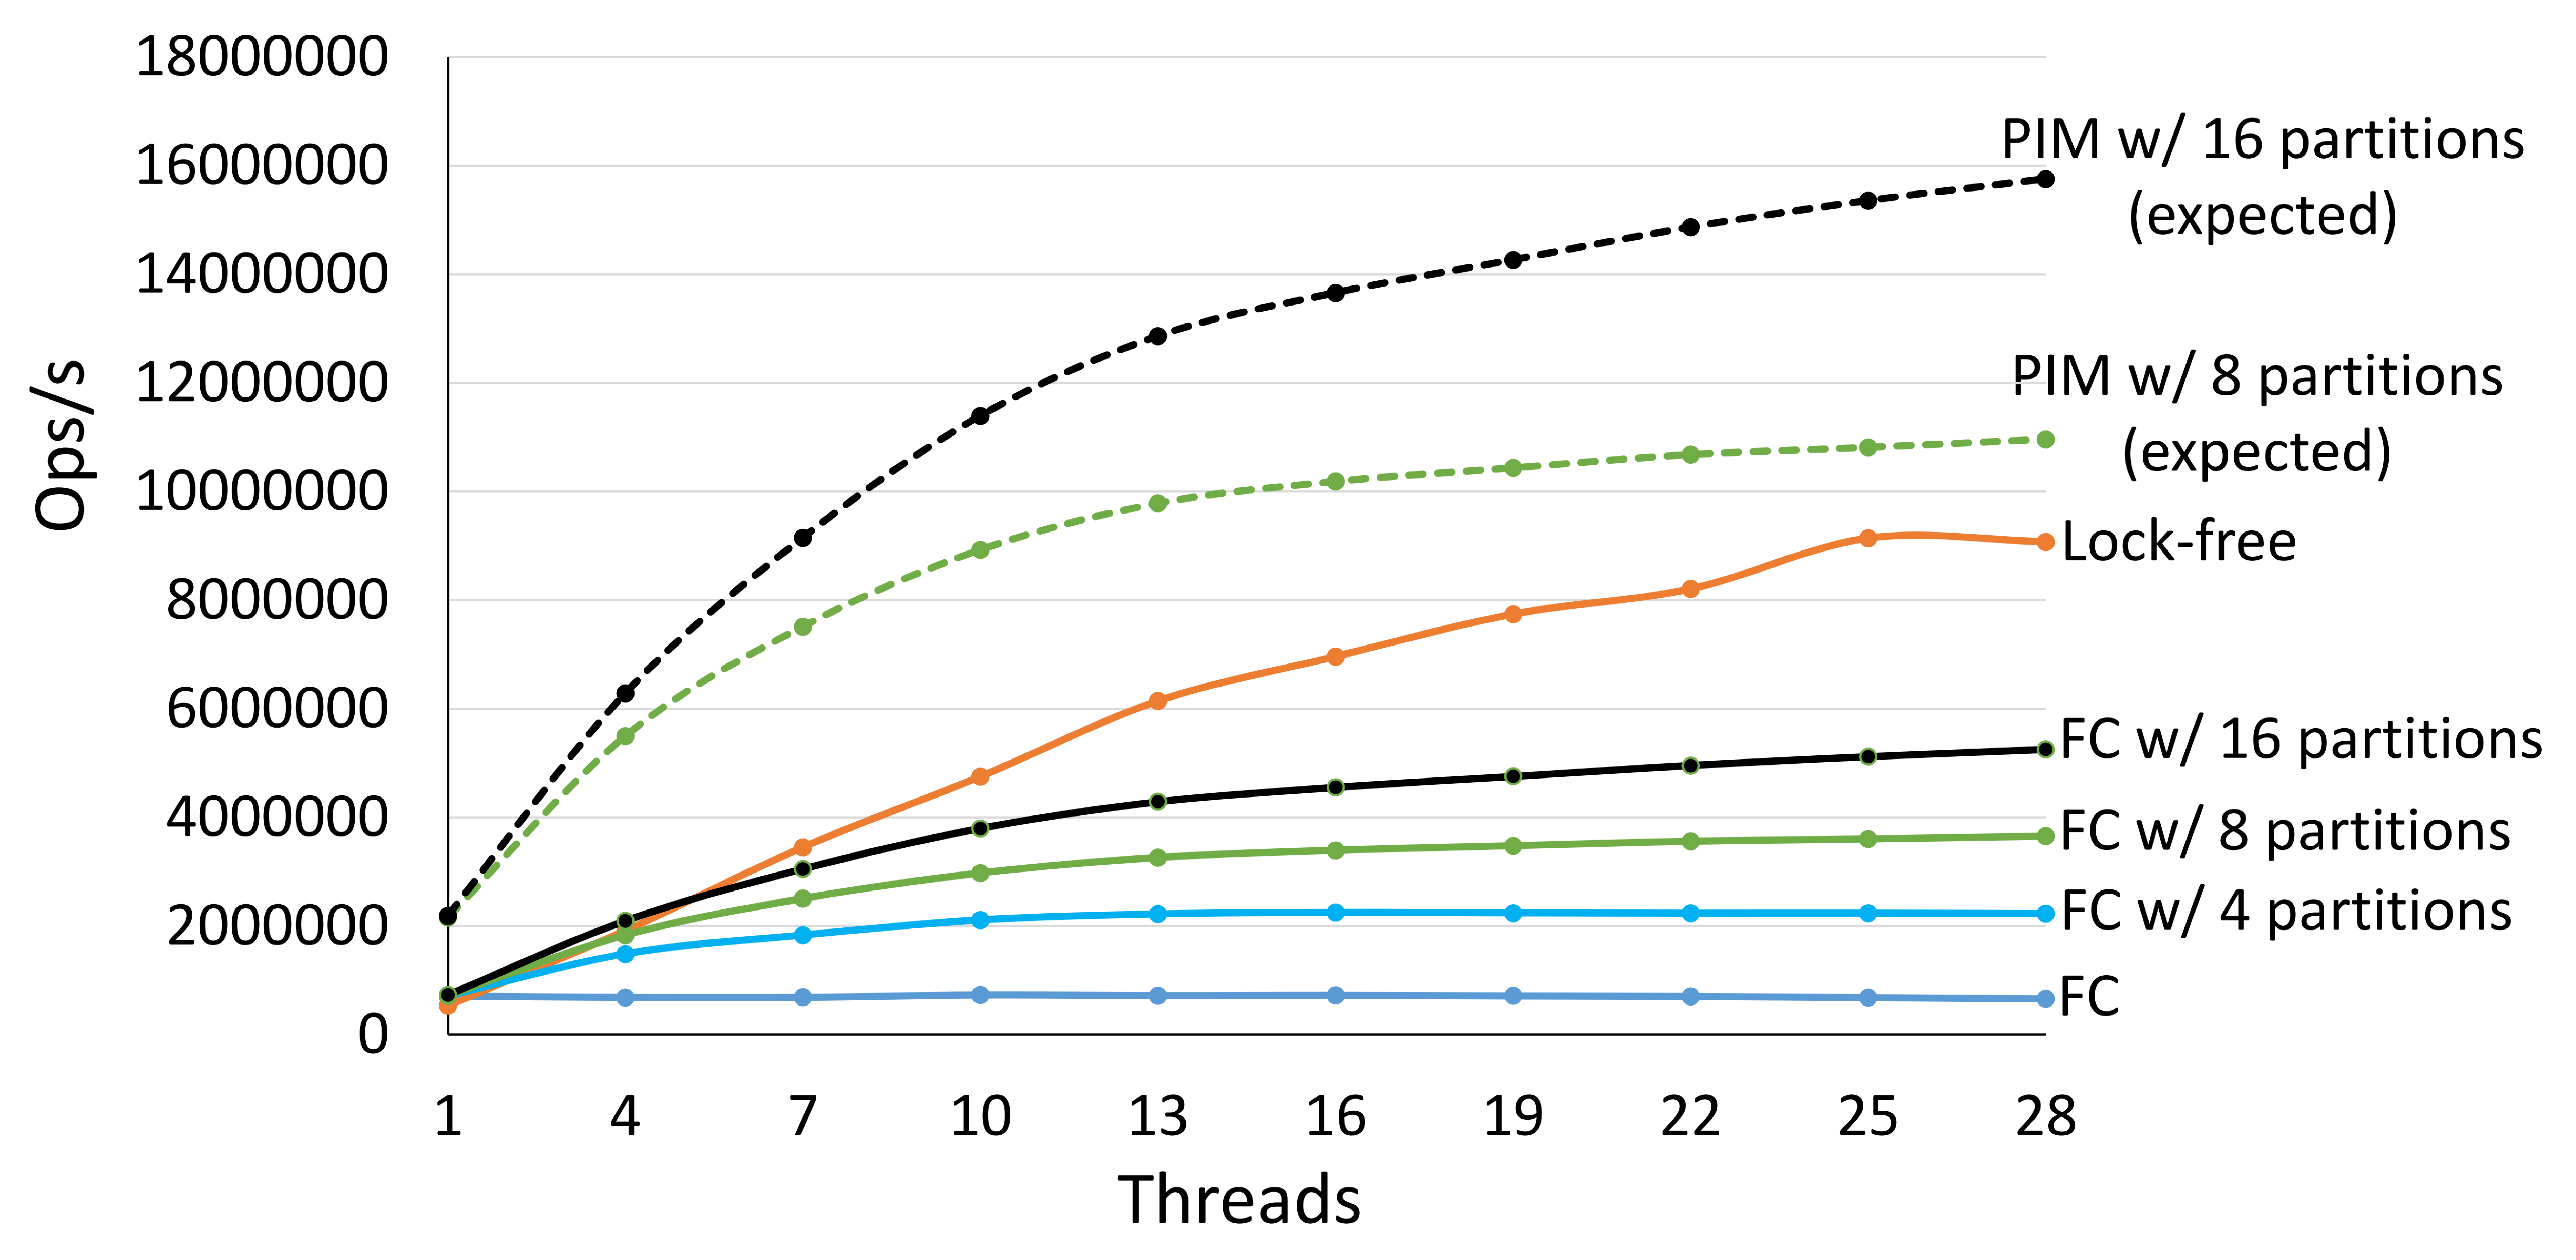
\includegraphics[width=.98\textwidth]{skiplist_data.eps} % second figure itself
        \caption{Experimental results of skip-lists}
        \label{figure:skiplist_data}
    \end{minipage}
\end{figure}



\subsection{Skip-lists}
\label{section:skip_list}

%\subsubsection{Base algorithm}

Like the naive PIM-managed linked-list,
the naive PIM-managed skip-list keeps the skip-list in a single vault and
CPUs send operation requests to the local PIM core that executes those operations.
As we will see, this algorithm is less efficient than some existing algorithms.

Unfortunately, the combining optimization cannot be applied to skip-lists effectively.
The reason is that for any two nodes not close enough to each other in the skip-list,
the paths we traverse through to reach them don't largely overlap.

On the other hand, PIM memory usually consists of many vaults and PIM cores.
For instance, the first generation of Hybrid Memory Cube \cite{website:HMC} has up to 32 vaults.
Hence, a PIM-managed skip-list may achieve much better performance if
we can exploit the parallelism of multiple vaults.
Here we present our PIM-managed skip-list with a \textit{partitioning optimization}:
A skip-list is divided into partitions of disjoint ranges of keys,
stored in different vaults, so that a CPU sends its operation request to
the PIM core of the vault to which the key of the operation belongs.

Figure \ref{figure:skiplist_structure} illustrates the structure of a PIM-managed skip-list.
Each partition of a skip-list starts with a \textit{sentinel node}
which is a node of the max height. 
For simplicity, assume the max height $H_{max}$ is predefined.
A partition covers a key range between the key of its sentinel node and
the key of the sentinel node of the next partition.
CPUs also store a copy of each sentinel node in the normal DRAM and 
the copy has an extra variable indicating the vault containing the sentinel node.
Since the number of nodes of the max height is very small with high probability, 
those copies of those sentinel nodes can almost certainly stay in cache
if CPUs access them frequently.

When a CPU applies an operation for a key to the skip-list,
it first compares the key with those of the sentinels, discovers which vault
the key belongs to, and then sends its operation request to that vault's PIM core.
Once the PIM core retrieves the request, it executes the operation in the local vault 
and finally sends the result back to the CPU.


\begin{figure}[ht!]
%$\hrulefill$
%\\
%\\
\centering
\includegraphics[width=.6\linewidth]{skiplist_structure.eps}
%$\hrulefill$
\caption{A PIM-managed FIFO queue with three partitions}
\label{figure:skiplist_structure}
\end{figure}

Now let us discuss how we implement the PIM-managed skip-list
when the key of each operation is an integer generated uniformly at random
from range $[0, n]$ and the PIM memory has $k$ vaults available.
Initially we can create $k$ partitions starting with fake sentinel nodes
with keys $0, 1/k, 2/k,..., (n-1)/k$, respectively, 
and allocate each partition in a different vault. 
The sentinel nodes will never be deleted.
If a new node to be added has the same key as a sentinel node,
we insert it immediately after the sentinel node.

We compare the performance of our PIM-managed skip-list with partitions 
to the performance of a flat-combining skip-list \cite{Hendler10}
and a lock-free skip-list \cite{Herlihy08}, 
where $p$ CPUs keeps making operation requests.
We also apply the partitioning optimization to the flat-combining skip-list, 
so that $k$ combiners are in charge of $k$ partitions of the skip-list. 
To simplify the comparison, we assume that all skip-lists have the same
initial structure (expect that skip-lists with partitions have extra sentinel nodes)
and all the operations are contains() operations
(or the number of $add()$ requests is the same as the number of $delete()$ 
so that the size of each skip-list nearly doesn't change).
Their approximate expected throughputs are as follows:
\begin{itemize}
\item Look-free skip-list:
	${p \over \beta\latcpu}$

\item Flat-combining skip-list without partitioning:
	${1 \over \beta\latcpu}$

\item PIM-managed skip-list without partitioning:
	${1 \over (\beta\latpim + \latmes)}$

\item Flat-combining skip-list with $k$ partitions:
    ${k \over \beta\latcpu}$

\item PIM-managed linked-list with $k$ partitions:
    ${k \over (\beta\latpim + \latmes)}$
\end{itemize}
where $\beta$ is the average number of nodes an operation has to go through
in order to find the location of its key in a skip-list
($\beta = \Theta(\log N)$, where $N$ is the size of the skip-list).
Note that we have ignored some overheads in the flat-combining
algorithms, such as maintaining combiner locks and publication lists
(we will discuss publication lists in more detail in Section \ref{section:contended}).
We also have overestimated the performance of the lock-free skip-list by not counting the
CAS operations used in add() and delete() requests, as well as the cost of retries
caused by conflicts of updates.
Even so, our PIM-managed linked-list with partitioning optimization is
still expected to outperform the second best algorithm, the lock-free skip-list 
when $k > {(\beta\latpim + \latmes)p \over \beta\latcpu}$.
Given that $\latmes = \latcpu = 3\latpim$, $k > p/3$ should suffice.

Our experiments have revealed similar results, 
as presented in Figure \ref{figure:skiplist_data}.
We have implemented and run the flat-combining skip-list with different numbers of
partitions and compared them with the lock-free skip-list.
As the number of partitions increases, the performance of the flat-combining skip-list
gets better, implying the effectiveness of the partitioning optimization.
Again we believe the performance of the flat-combining skip-list is a good indicator
to the performance of our PIM-managed skip-list.
Therefore, according to the analytical results we have shown, we can triple the throughput
of a flat-combining skip-list to get the expected performance of a PIM-managed skip-list.
As the figure illustrates, when the PIM-managed skip-list has $8$ or $16$ partitions,
it is expected to outperform the lock-free skip-list with up to 28 hardware threads.


%\subsubsection{Rebalancing skip-list}
\subsection{Skip-list Rebalancing}
We have shown that our PIM-managed skip-list performs well with uniform distribution of requests. 
With non-uniform distribution of requests, we may need to periodically rebalance the skip-list 
in order to maintain good performance. 
To do so, we can migrate consecutive nodes from one vault to another without blocking requests.  

To move consecutive nodes from its local vault to another vault $v$, a PIM core $p$ 
can send messages requesting those nodes to be added to the local PIM core $q$ of $v$ as follows. 
First, $p$ sends a message notifying $q$ of the start of the migration. 
Then $p$ sends messages of adding those nodes to $q$ one by one in an ascending order 
according to the keys of the nodes. 
After all those nodes have been migrated, $p$ sends notification messages to CPUs so that 
CPUs can update their copies of sentinel nodes accordingly.
Once $p$ receives acknowledgement messages from all CPUs, it notifies $q$ of the end of migration.
To keep the node migration protocol simple, we don't allow $q$ to move those nodes 
to another vault again until $p$ finishes its node migration. 

During this node migration, $p$ can still periodically check its message buffer for requests from CPUs.
Assume that a request with key $k_1$ is sent to $p$ when $p$ is migrating nodes 
in a key range containing $k_1$.  
If $p$ is about to migrate a node with $k_2$ at the moment and $k_1 \ge k_2$, 
$p$ serves the request itself. 
Otherwise $p$ forwards the request to $q$. 
In either case, $p$ can then continue its node migration without blocking concurrent requests. 
This algorithm is correct in the presence of requests, because 
a request will eventually reach the vault that 
currently contains nodes in the key range that the request belongs to: 
If a request arrives to $p$ which no longer holds the partition the request belongs to, 
$p$ can simply reply with a rejection to the CPU and the CPU will resend its request to 
the correct PIM core, 
because it has already updated its sentinels and knows which PIM core it should contact now. 

Using this node migration protocol, our FIFO queue can support two rebalancing schemes:
1) If a partition has too many nodes, the local PIM core can divide it into two smaller  
partitions and migrate one of them to another PIM vault; 
2) If two consecutive partitions are both small, 
we can merge then by moving one to the vault containing the other. 
If rebalancing happens infrequently, its overhead is affordable. 



%\section{Contended Data Structures}
\section{High Contention Data Structures}
\label{section:contended}
In this section, we consider data structures that are often contended when accessed 
by many threads concurrently. In these data structures, operations compete for accessing one or several 
locations, creating a contention spot, which can become a performance bottleneck.
Examples include head and tail pointers in queues or the top pointer of a stack.

These data structures have good locality and the contention spots are often found 
in shared CPU caches, such as the last level cache in a multi-socket non-uniform memory access machine 
when accessed by threads running only on one socket. Therefore, these data structures might 
seem to be a poor fit for near-memory computing, because the advantage of the faster access to memory is 
muted by having the frequently accessed data in the cache. 
However, such a perspective does not 
consider the overhead introduced by contention in a concurrent data structure where all threads 
try to access the same locations. 

As a representative example of this class of data structures, we consider a FIFO queue, 
where concurrent enqueue
and dequeue operations compete for the head and tail of the queue, respectively. 
Although a naive PIM FIFO queue is not a good replacement for a well crafted concurrent FIFO queue, 
we show that, counterintuitively, PIM can still have benefits over a traditional concurrent FIFO 
queue. In particular, we exploit the pipelining of requests from CPUs, which can be done very efficiently in PIM, to 
design a PIM FIFO queue that can outperform state-of-the-art concurrent FIFO queues, such as the one using flat combining~\cite{Hendler10} 
and the one using fetch and add~\cite{Morrison13}.

\subsection{FIFO queues}
The structure of our PIM-managed FIFO queue is shown in Figure \ref{figure:queue_structure}.
A queue consists of a sequence of segments, each containing consecutive nodes of the queue.
A segment is allocated in a PIM vault, with a head node and a tail node pointing to the first 
and the last nodes of the segment, respectively.
A vault can contain multiple (mostly likely non-consecutive) segments. 
There are two special segments---the \textit{enqueue segment} and the \textit{dequeue segment}.
To enqueue a node, a CPU sends an enqueue request to the PIM core of the vault 
containing the enqueue segment.
The PIM core will then insert the node to the head of the segment.
Similarly, to dequeue a node, a CPU sends a dequeue request to the PIM core of the vault
holding the dequeue segment. 
The PIM core will then pop out the node at the tail of the dequeue segment and 
send the node back to the CPU.

\begin{figure}[ht!]
%$\hrulefill$
%\\
%\\
\centering
\includegraphics[width=1.0\linewidth]{queue_structure.eps}
%$\hrulefill$
\caption{A PIM-managed FIFO queue with three segments}
\label{figure:queue_structure}
\end{figure}

Initially the queue consists of an empty segment which acts as both the enqueue segment and 
the dequeue segment. 
When the length of enqueue segment exceeds some threshold, the PIM core maintaining it
notifies another PIM core to create a new segment as the new enqueue segment.\footnote{
Alternative designs are also possible and the decision can also be made by CPUs,
based on more complex criteria. We omit these alternatives for briefness.}
When the dequeue segment becomes empty and the queue has other segments, 
the dequeue segment is deleted and the segment that was created first 
among all the remaining segments is designated as the new dequeue segment. 
This segment was created when the old dequeue segment 
acted as the enqueue segment and exceeded the length threshold.
If the enqueue segment is different from the dequeue segment, 
enqueue and dequeue operations can be executed by two different PIM cores 
in parallel, which doubles the throughput compared to a straightforward queue implementation 
held in a single vault.  


\begin{algorithm*}[ht!]
{\footnotesize
%scriptsize
\caption{PIM-managed FIFO queue}
\label{alg:queue}
\vspace{-2.5ex}
\begin{multicols}{2}
\begin{algorithmic}[1]
\Procedure{enq}{cid, $u$}
	\If{enqSeg == null}
        \State send message(cid, false);
    \Else
        \If{enqSeg.head $\ne$ null}
            \State enqSeg.head.next = $u$;
            \State enqSeg.head = $u$;
        \Else
            \State enqSeg.head = $u$;
            \State enqSeg.tail = $u$;
        \EndIf

        \State enqSeg.count = enqSeg.count + 1;
        \State send message(cid, true);

        \If{enqSeg.count $>$ threshold}
            \State cid$'$ = the CID of the PIM core chosen to maintain the new segment;
            \State send message(cid$'$, newEnqSeg());
            \State enqSeg.nextSegCid = cid$'$;
            \State enqSeg = null;
        \EndIf
    \EndIf
\item[]
\EndProcedure
\end{algorithmic}

\begin{algorithmic}[1]
\Procedure{newEnqSeg}{\null}
	\State enqSeg = new Segment();
	\State segQueue.enq(engSeg) ;
	\State notify CPUs of the new enqueue segment;
\EndProcedure
\end{algorithmic}

\columnbreak

\begin{algorithmic}[1]
\Procedure{deq}{cid}
	\If{deqSeg == null}
        \State send message(cid, false);
    \Else
        \If {deqSeg.tail $\ne$ null}
			\State send message(cid, deqSeg.tail);
            \State deqSeg.tail = deqSeg.tail.next;   
        \Else
			\If {deqSeg == enqSeg}
				\State send message(cid, null);
			\Else
                \State send message(deqSeg.nextSegCid, newDeqSeg());
                \State deqSeg = null;
                \State send message(cid, false);
            \EndIf            
        \EndIf 
    \EndIf     
\item[]
%\item[]
%\item[]
%\item[]
%\item[]
\EndProcedure
\end{algorithmic}


\begin{algorithmic}[1]
\Procedure{newDeqSeg}{\null}
	\State deqSeg = segQueue.deq();
	\State notify CPUs of the new dequeue segment; 
\EndProcedure
\end{algorithmic}

\end{multicols}
}
\vspace{-2ex}
\end{algorithm*}


The pseudocode of the algorithm is presented in Algorithm \ref{alg:queue}. 
Each PIM core has local variables enqSeg and deqSeg that are references to 
local enqueue and dequeue segments.
When enqSeg (respectively deqSeq) is not null, it indicates that the PIM core is currently 
holding the enqueue (respectively dequeue) segment.
Each PIM core also maintains a local queue segQueue for storing local segments.
CPUs and PIM cores communicate via message(cid, content) calls, where cid is the unique core ID (CID) 
of the receiver and the content is either a request or a response to a request.

Once a PIM core receives an enqueue request enq(cid, $u$) of node $u$ from a CPU whose CID is cid,
it first checks if it is holding the enqueue segment (line 2 of Procedure enq(cid, $u$)).
If so, the PIM core enqueues $u$ (lines 5-12), and otherwise sends back a message
informing the CPU that the request is rejected (line 3) so that
the CPU can resend its request to the right PIM core holding the enqueue segment
(we will explain later how the CPU can find the right PIM core).
After enqueuing $u$, the PIM core may find the enqueue segment is longer than the threshold (line 13).
If so, it sends a message with a newEnqSeg() request to the PIM core of another vault that is chosen 
to create a new enqueue segment.
Finally the PIM core sets its enqSeq to null indicating it no longer deals with enqueue operations.
Note that the CID \emph{cid} of the PIM core chosen for creating the new segment is recorded in 
enqSeg.nextSegCid for future use in dequeue requests.
As Procedure newEnqSeg() in Algorithm \ref{alg:queue} shows,
The PIM core receiving this newEnqSeg() request creates a new enqueue segment and enqueues 
the segment into its segQueue (line 3). 
Finally it notifies CPUs of the new enqueue segment (we will get to it in more detail later).

Similarly, when a PIM core receives a dequeue request deq(cid) from a CPU with CID \emph{cid},
it first checks whether it still holds the dequeue segment (line 2 of Procedure deq(cid)).
If so, the PIM core dequeues a node and sends it back to the CPU (lines 5-7).
Otherwise, it informs the CPU that this request has failed (line 3) and
the CPU will have to resend its request to the right PIM core.
If the dequeue segment is empty (line 8) and the dequeue segment is not the same as 
the enqueue segment (line 11), which indicates that the FIFO queue is not empty 
and there exists another segment, the PIM core sends a message with a newDeqSeg() request 
to the PIM core with CID \emph{deqSeg.nextSegCid}. 
(We know that this PIM core must hold the next segment, 
according to how we create new segments in enqueue operations, 
as shown at lines 14-16 of Procedure enq(cid, $u$).) 
Upon receiving the newDeqSeg() request, as illustrated in Procedure newDeqSeg(), 
the PIM core retrieves from its segQueue the oldest segment it has created and 
makes it the new dequeue segment (line 2). 
Finally the PIM core notifies the CPU that it is holding the new dequeue segment now.

Now we explain how CPUs and PIM cores coordinate to make sure that CPUs can find the right enqueue 
and dequeue segments, when their previous attempts have failed due to changes of those segments. 
We will only discuss how to deal with enqueue segments here, 
since the same methods can be applied to dequeue segments. 
A straightforward way to inform CPUs is to have the owner PIM core of the new enqueue segment 
send notification messages to them (line 4 of newEngSeg()) 
and wait until CPUs all send back acknowledgement messages. 
However, if there is a slow CPU that doesn't reply in time, 
the PIM core has to wait for it and therefore other CPUs cannot have their requests executed. 
A more efficient, non-blocking method is to have the PIM core start working for new requests 
immediately after it has sent off those notifications. 
A CPU does not have to reply to those notifications in this case, 
but if its request later fails, it needs to send messages to (sometimes all) PIM cores 
to ask whether a PIM core is currently in charge of the enqueue segment.
In either case, the correctness of the algorithm is guaranteed:  
at any time, there is only one enqueue segment and only one dequeue segment, 
and only requests sent to them will be executed. 
  
We would like to mention that the PIM-managed FIFO can be further optimized. 
For example, the PIM core holding the enqueue segment can combine multiple pending enqueue requests 
and store the nodes to be enqueued in an array as a ``fat" node of the queue, 
so as to reduce memory accesses. 
This optimization is also used in the flat-combining FIFO queue \cite{Hendler10}. 
Even without this optimization, our algorithm still performs well, as we will show next. 

\subsection{Pipelining and Performance analysis}
We compare the performance of three concurrent FIFO queue algorithms---our PIM-manged FIFO queue, 
a flat-combining FIFO queue and a F\&A-based FIFO queue \cite{Morrison13}. 
The F\&A-based FIFO queue is the most efficient concurrent FIFO queue we are aware of, 
where threads make F\&A operations on two shared variables, 
one for enqueues and the other for dequeues, to compete for slots in the FIFO queue to 
enqueue and dequeue nodes (see \cite{Morrison13} for more details). 
The flat-combining FIFO queue we consider is based on the one proposed by \cite{Hendler10}, 
with a modification that threads compete for two ``combiner locks", 
one for enqueues and the other for dequeues. 
We further simplify it based on the assumption that the queue is always non-empty, 
so that it doesn't have to deal with synchronization issues between enqueues and dequeues 
when the queue is empty. 

Let us first assume that a queue is long enough such that the PIM-managed FIFO queue 
has more than one segment, and enqueue and dequeue requests can be executed separately. 
Since changes of enqueue and dequeue segments happen very infrequently, 
its overhead is negligible and therefore ignored to simplify our analysis.
(If the threshold of segment length at line 13 of enq(cid, $u$) is a large integer $n$, 
then, in the worst case, changing an enqueue or dequeue segment happens only once every $n$ requests, 
and the cost is only the latency of sending one message and a few steps of local computation.)
Since enqueues and dequeues are isolated in all the three algorithms when queues are long enough, 
we will focus on dequeues, and the analysis of enqueues is almost identical. 

Assume there are $p$ concurrent dequeue requests by $p$ threads. 
Since each thread needs to make a F\&A operation on a shared variable in the F\&A-based algorithm 
and F\&A operations on a shared variable are essentially serialized, 
the execution time of $p$ requests in the algorithm is at least $p\latato$. 
If we assume that each CPU makes a request immediately after its previous request completes, 
we can prove that the throughput of the algorithm is at most ${1 \over \latato}$. 

The flat-combining FIFO queue maintains a sequential FIFO queue and 
threads submit their requests into a publication list. 
The publication list consists of slots, one for each thread, to store those requests.
After writing a request into the list, a thread competes with other threads for acquiring a lock 
to become the ``combiner". 
The combiner then goes through the publication list to retrieve requests, executes operations for 
those requests and writes results back to the list, while other threads spin on their slots, 
waiting for the results. 
The combiner therefore makes two last-level cache accesses to each slot other than its own slot, 
one for reading the request and one for writing the result back. 
Thus, the execution time of $p$ requests in the algorithm is at least $(2p-1)\latllc$ and 
the throughput of the algorithm is roughly ${1 \over 2\latllc}$ for large enough $p$.

Note that we have made quite optimistic analysis for the F\&A-based and flat-combining algorithms 
by counting only the costs in part of their executions. 
The latency of accessing and modifying queue nodes in the two algorithms is ignored here. 
For dequeues, this latency can be high: since nodes to be dequeued in a long queue is unlikely 
to be cached, the combiner has to make a sequence of memory accesses to dequeue them one by one.  
Moreover, the F\&A-based algorithm may also suffer performance degradation under heavy contention, 
because contended F\&A operations may perform worse in practice.

\begin{figure}[ht!]
%$\hrulefill$
%\\
%\\
\centering
\subfigure[]{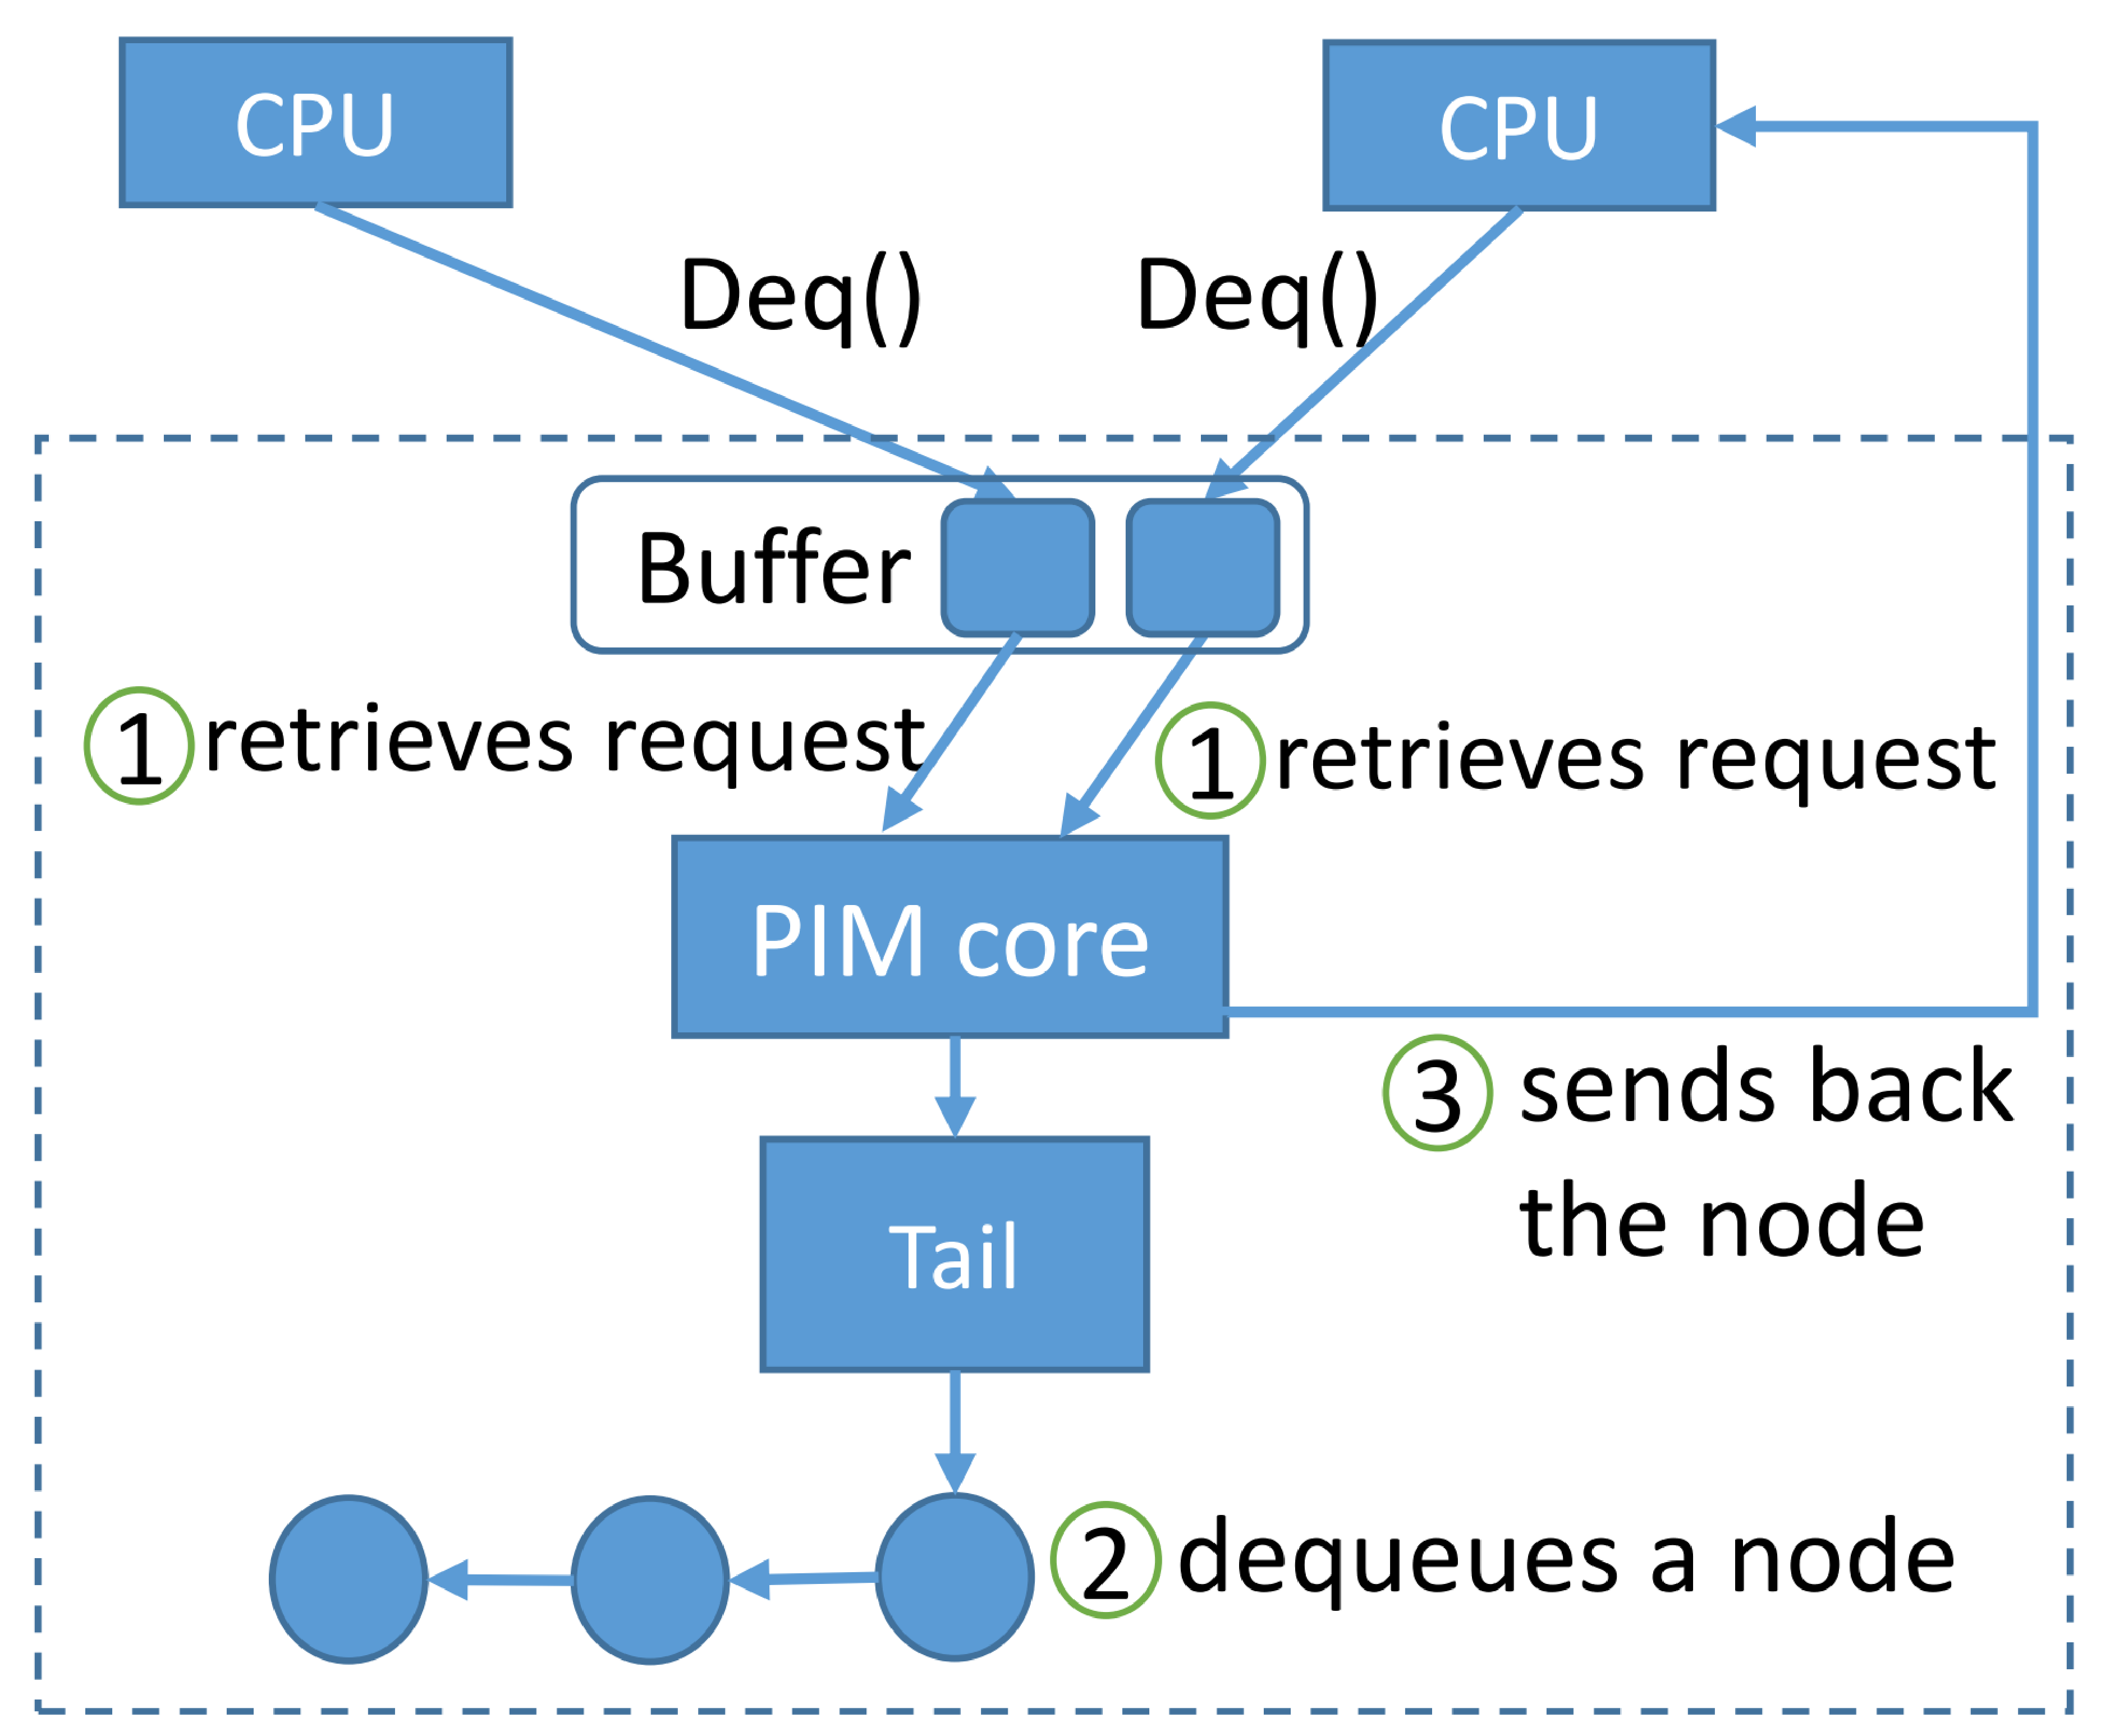
\includegraphics[width=.8\linewidth]{queue_pipeline.eps}}
\\
\subfigure[]{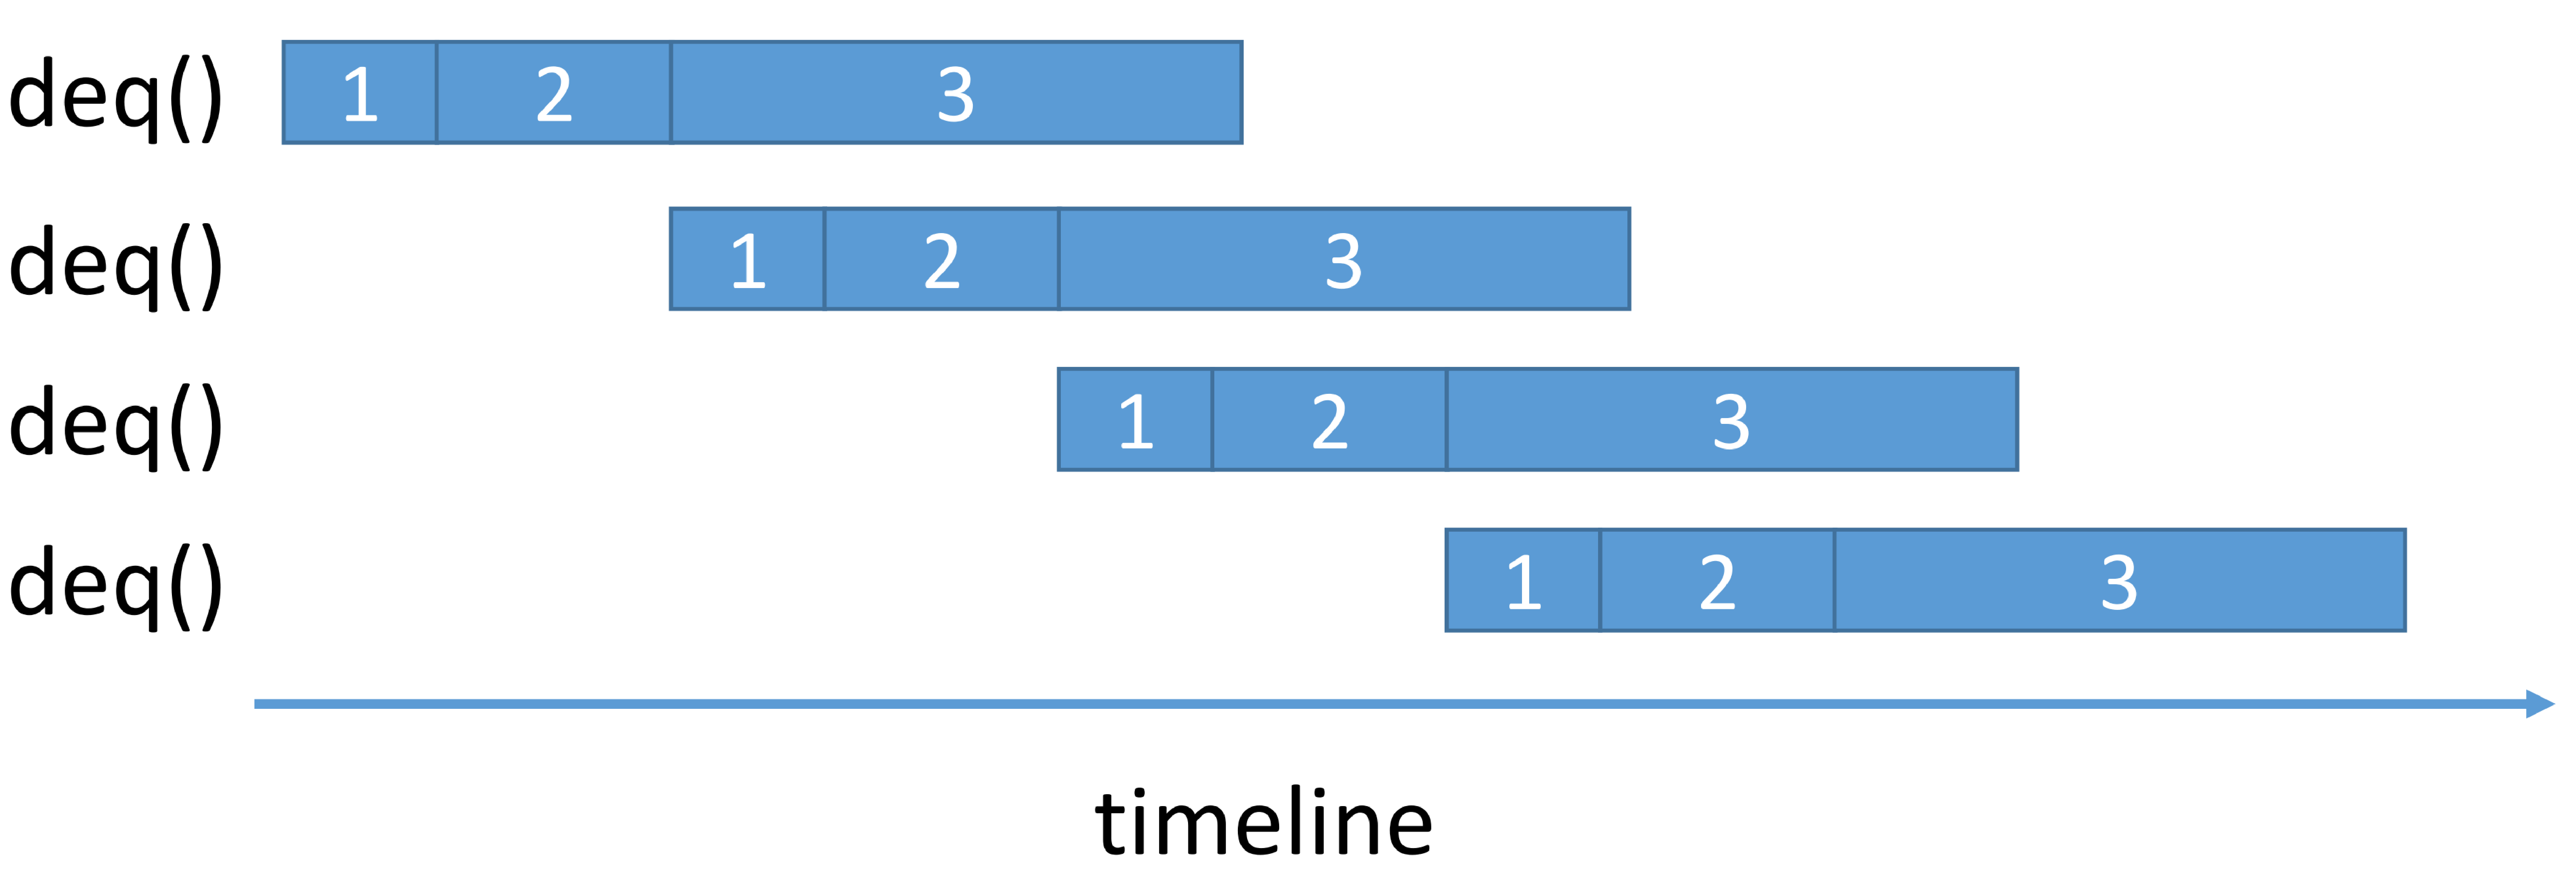
\includegraphics[width=1.0\linewidth]{queue_pipeline_timeline.eps}}

%$\hrulefill$
\caption{(a) illustrates the pipelining optimization, where a PIM core can start executing 
a new deq() (step 1 of deq() for the CPU on the left), without waiting for the dequeued node of 
the previous deq() to return to the CPU on the right (step 3). 
(b) shows the timeline of pipelining four deq() requests.}
\label{figure:queue_pipeline}
\end{figure}

The performance of our PIM-managed FIFO queue seems poor at first sight: although a PIM core can update 
the queue efficiently, it takes a lot of time for the PIM core to send results back to CPUs one by one. 
To improve its performance, the PIM core can \textit{pipeline} the executions of requests, 
as illustrated in Figure \ref{figure:queue_pipeline}(a). 
Suppose $p$ CPUs send $p$ dequeue requests concurrently to the PIM core, which takes time $\latmes$. 
The PIM core then retrieves a request from its message buffer (step 1 in the figure), 
dequeues a node (step 2) for the request, and sends the node back to the CPU (step 3). 
Here is how we hide the message latency in step 3: 
after sending off the message containing the node in step 3, the PIM core immediately retrieves the next 
request to execute, without blocking to wait for that message to arrive at its receiver. 
This way, the PIM core pipelines requests by overlapping the latency of message transfer in step 3  
and the latency of memory accesses and local computations in steps 1 and 2 in multiple requests 
(see Figure \ref{figure:queue_pipeline}(b)). 
Note that the PIM core still executes everything sequentially, 
as it always first sends off the message for the current request before serving the next.
 
The throughput of the PIM core is eventually decided by the costs of its memory accesses and local operations, 
as long as it has enough bandwidth to keep sending off messages,  
which is the case for this algorithm, because only one message is sent per request.
More specifically, as Figure \ref{figure:queue_pipeline}(b) illustrates, 
the total execution time of $p$ requests is the sum of the execution times of the first two steps 
for the $p$ requests, plus the message transfer time of step 3 for the last request.   
Since the PIM core in the execution of a dequeue only makes one memory access to read the node 
to be dequeued, and two L1 cache accesses to read and modify the tail node of the dequeue segment,   
the execution time of $p$ requests, including the time CPUs send their requests to the PIM core, 
is only $\latmes + p(\latpim + \epsilon) + \latmes$, where $\epsilon$ 
is the total latency of the PIM core making two L1 cache accesses and sending off one message, 
which is negligible in our performance model. 

Assume that each CPU makes another request immediately after it receives the result of its previous request 
and that there are enough (at least $2\latmes / \latpim$) CPUs sending requests.
We can prove that the PIM core can always find another request in its buffer after it executes one. 
Thus by the same analysis as above, we have $\latmes + x(\latpim + \epsilon) + \latmes = 1$, 
where $x$ is the throughput of the PIM core in one second. 
Therefore, the throughput of the PIM-managed FIFO queue is approximately 
$${1 - 2\latmes \over \latpim + \epsilon} \approx {1 - 2\latmes \over \latpim} 
\approx {1 \over \latpim},$$
since $\latmes$ is usually only hundreds of nanoseconds. 

Comparing the throughputs of the three FIFO queue algorithms, 
we can conclude that the PIM-managed FIFO queue with pipelining outperforms the other two algorithms 
when $2r_1 / r_2$ and $r_1 r_3$. 
If we assume $r_1 = r_2 = 3$ and $r_3 = 1$, then the throughput of our FIFO queue is expected 
twice the throughput of the flat-combining queue and three times that of the F\&A queue. 

When the PIM-managed FIFO queue is short, it may contain only one segment 
which deals with both enqueue and dequeue requests. 
In this case, its throughput is only half of the throughput shown above, 
but it should still be at least as good as the throughput of the other two algorithms. 


\section{Related Work}

Researchers have studied the PIM model for decades (e.g., \cite{Stone1970, Kogge1994, 
Gokhale1995, Patterson1997, Oskin1998, KangHYKGLTP99, Hall1999}). 
Implementations of PIM memory have become much more feasible recently due to the advancements 
in 3D-stacked technology that can stack memory dies on top of a logic layer 
\cite{jeddeloh2012, Loh2008, Black2006}. 
Based on this technology, Micron and other vendors together implemented a prototype of 
PIM memory called the Hybrid Memory Cube \cite{website:HMC} a few years ago. 
Since then, the PIM model has drawn a lot of attention in the computer architecture community. 
Different PIM-based architectures have been proposed, either for general purposes or for 
specific applications \cite{Ahn2015:1, Ahn2015:2, Zhang2014:TTP, hsieh2016accelerating,
Azarkhish16, Akin2015:DRM, Azarkhish2015, AzarkhishPRLB17, boroumand2016, ZhuASSHPF13, ZhuGSPF13}.

Besides PIM memory's low energy consumption and high bandwidth 
(e.g., \cite{Ahn2015:2, Zhang2014:TTP, ZhuASSHPF13, AzarkhishPRLB17}), 
researchers have also explored the benefits of PIM memory's low memory access latency
\cite{Loh2008, hsieh2016accelerating, Azarkhish16}, which is what we focus on in this paper. 
To our knowledge, however, we are the first to utilize PIM memory for designing efficient 
concurrent data structures. 
Although some researchers have studied how PIM memory can help speed up concurrent 
operations to data structures, such as parallel graph processing \cite{Ahn2015:2} and  
parallel pointer chasing on linked data structures \cite{hsieh2016accelerating}, 
the applications they consider require very simple, if any, synchronization between operations. 
In contract, operations to concurrent data structures can interleave in arbitrary orders, 
and therefore they have to correctly synchronize with one another in all possible situations. 
This makes designing concurrent data structures with correctness guarantees like 
linearizability \cite{Herlihy90} very challenging. 

Moreover, no one has ever compared the performance of data structures in the PIM model 
with that of existing concurrent data structures in the classic shared memory model. 
We analyze and evaluate concurrent linked-lists and skip-lists, 
as representatives of pointer-chasing data structures, and concurrent FIFO queues, 
as representatives of contended data structures.
For linked-lists, we compare our PIM-managed implementation with the concurrent linked-list with 
fine-grained locks \cite{Heller05}, and the one implemented using flat combining 
\cite{Hendler10}, a generic technique to design concurrent data structures.  
For skip-lists, we compare our implementation with the lock-free skip-list \cite{Herlihy08} 
and a skip-list with flat combining and partitioning optimization. 
For FIFO queues, we compare our implementation with the flat-combining FIFO queue 
\cite{Hendler10} and the F\&A-based FIFO queue \cite{Morrison13}.  
As we will show in the paper, our simple PIM-managed concurrent data structures can in theory 
outperform those concurrent data structures, 
making PIM memory a promising platform to run concurrent data structures.
\section{Conclusion}
\label{section:conclusion}
In this paper, we study how to exploit the low access latency 
of PIM memory to design efficient concurrent data structures for the PIM memory.
To analyze and compare the performance of our PIM-managed data structures with 
concurrent data structures in the literature, we propose a simplified 
performance model based on the latencies assumed by prior work on PIM
memory and on current multiprocessor architectures. 
We show that sequential PIM data structures cannot outperform traditional 
concurrent data structures, 
due to the lack of parallelism and the high communication cost between the CPUs and the PIM 
cores.  
To improve the performance of PIM data structures, we propose novel designs for    
low contention 
pointer-chasing data structures, such as linked-lists and skip-lists, and for high-contention  
data structures, such as FIFO queues. 
We show that our PIM algorithms can outperform state-of-the-art concurrent 
data structures, making PIM memory a promising platform for managing data structures.

 

%\bibliographystyle{ACM-Reference-Format}
\bibliographystyle{plain}
\bibliography{refs_pim}

\end{document}

